\documentclass[tikz,border=6pt]{standalone}
\usepackage{tikz}
\usetikzlibrary{arrows.meta}
\definecolor{nebula}{HTML}{6366F1}
\definecolor{spark}{HTML}{14B8A6}
\definecolor{ink}{HTML}{334155}
\begin{document}
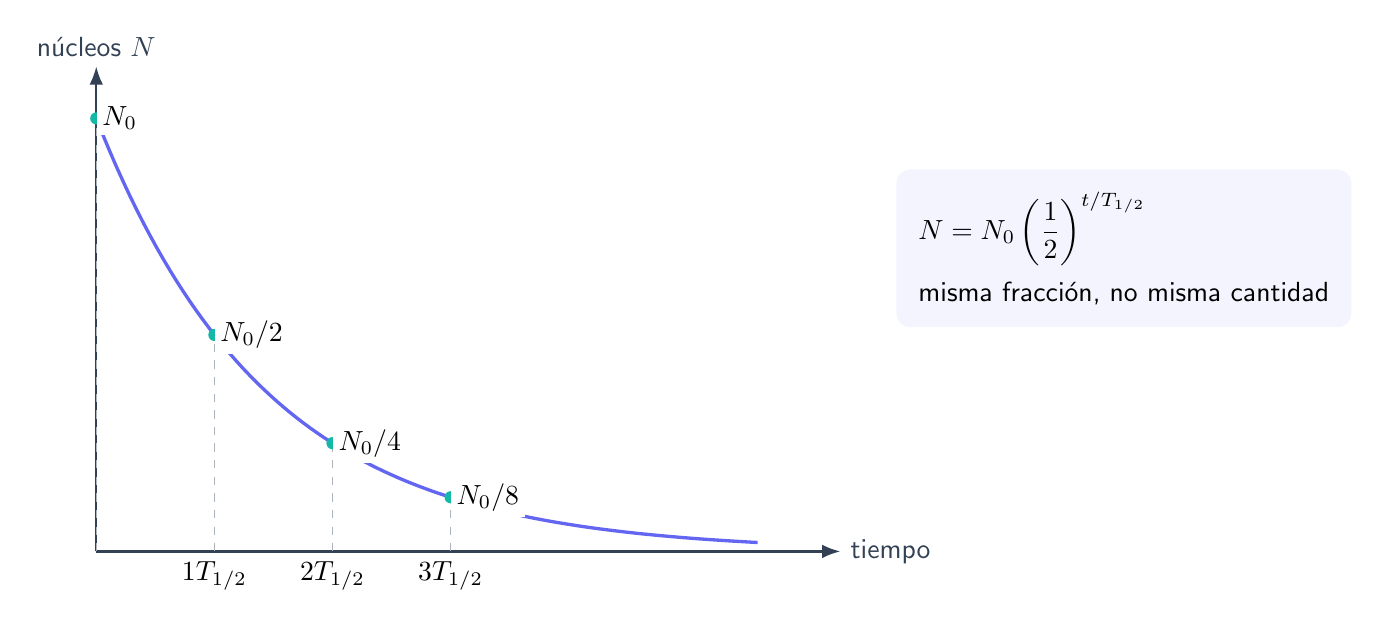
\begin{tikzpicture}[font=\sffamily,>=Latex,x=1.5cm,y=0.055cm]
  \draw[->,thick,ink] (0,0)--(6.3,0) node[right] {tiempo};
  \draw[->,thick,ink] (0,0)--(0,112) node[above] {n\'ucleos $N$};
  \draw[very thick,nebula,domain=0:5.6,samples=100] plot (\x,{100*exp(-0.693*\x)});
  \draw[dashed,ink!40] (0,0)--(0,100); \fill[spark] (0,100) circle(2.2pt); \node[fill=white,inner sep=2pt,right] at (0,100) {$N_0$};
  \draw[dashed,ink!40] (1,0)--(1,50); \fill[spark] (1,50) circle(2.2pt); \node[fill=white,inner sep=2pt,right] at (1,50) {$N_0/2$};
  \draw[dashed,ink!40] (2,0)--(2,25); \fill[spark] (2,25) circle(2.2pt); \node[fill=white,inner sep=2pt,right] at (2,25) {$N_0/4$};
  \draw[dashed,ink!40] (3,0)--(3,12.5); \fill[spark] (3,12.5) circle(2.2pt); \node[fill=white,inner sep=2pt,right] at (3,12.5) {$N_0/8$};
  \foreach \x in {1,2,3}{\node[below] at (\x,0) {$\x T_{1/2}$};}
  \node[align=left,fill=nebula!7,rounded corners=5pt,inner sep=8pt] at (8.7,70) {$\displaystyle N=N_0\left(\frac12\right)^{t/T_{1/2}}$\\[5pt]misma fracci\'on, no misma cantidad};
\end{tikzpicture}
\end{document}
